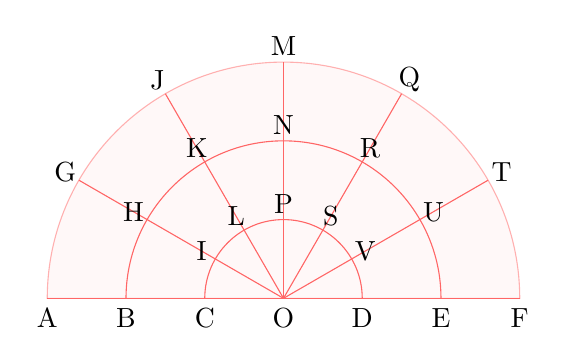
\begin{tikzpicture}	
  
    
\def \CharSize {1};
\def \BulletSize {1};


    %Définition de l 'angle de rotation de la figure
    \def \Rotation {0} 
    %Couleur des élèments de la figure (sauf le remplissage)
    \def \RapColor {red!60}


\begin{scope}[rotate=\Rotation]
    % contours
    \draw[color=\RapColor, fill =red!5, opacity=0.5] (-3,0) arc(180:0:3)--(3,0)--(-3,0)--cycle;	%Dont couleur de remplissage
    \draw[color=\RapColor] (-3,0)--(3,0);
    
   % demi-cercles intérieurs :
    \draw[color=\RapColor](-1,0) arc(180:0:1);
    \draw[color=\RapColor](-2,0) arc(180:0:2);
    
    
    % rayons :
   \foreach \a in {0,30,...,180}{\draw[color=\RapColor] (\a:3)--(\a:0);}
   
 
  
\end{scope}

\draw (0,0) node [below,scale=\CharSize]{O};
\draw (-3,0) node [below,scale=\CharSize]{A};
\draw (-2,0) node [below,scale=\CharSize]{B};
\draw (-1,0) node [below,scale=\CharSize]{C};
\draw (1,0) node [below,scale=\CharSize]{D};
\draw (2,0) node [below,scale=\CharSize]{E};
\draw (3,0) node [below,scale=\CharSize]{F};
\draw (150:3.2) node [scale=\CharSize]{G};
\draw (150:2.2) node [scale=\CharSize]{H};
\draw (150:1.2) node [scale=\CharSize]{I};
\draw (120:3.2) node [scale=\CharSize]{J};
\draw (120:2.2) node [scale=\CharSize]{K};
\draw (120:1.2) node [scale=\CharSize]{L};
\draw (90:3.2) node [scale=\CharSize]{M};
\draw (90:2.2) node [scale=\CharSize]{N};
\draw (90:1.2) node [scale=\CharSize]{P};
\draw (60:3.2) node [scale=\CharSize]{Q};
\draw (60:2.2) node [scale=\CharSize]{R};
\draw (60:1.2) node [scale=\CharSize]{S};
\draw (30:3.2) node [scale=\CharSize]{T};
\draw (30:2.2) node [scale=\CharSize]{U};
\draw (30:1.2) node [scale=\CharSize]{V};
    
\end{tikzpicture} 
